% Options for packages loaded elsewhere
% Options for packages loaded elsewhere
\PassOptionsToPackage{unicode}{hyperref}
\PassOptionsToPackage{hyphens}{url}
\PassOptionsToPackage{dvipsnames,svgnames,x11names}{xcolor}
%
\documentclass[
  default,
]{sn-jnl}


\usepackage{xcolor}
\usepackage{amsmath,amssymb}
\setcounter{secnumdepth}{5}
\usepackage{iftex}
\ifPDFTeX
  \usepackage[T1]{fontenc}
  \usepackage[utf8]{inputenc}
  \usepackage{textcomp} % provide euro and other symbols
\else % if luatex or xetex
  \usepackage{unicode-math} % this also loads fontspec
  \defaultfontfeatures{Scale=MatchLowercase}
  \defaultfontfeatures[\rmfamily]{Ligatures=TeX,Scale=1}
\fi
\usepackage{lmodern}
\ifPDFTeX\else
  % xetex/luatex font selection
\fi
% Use upquote if available, for straight quotes in verbatim environments
\IfFileExists{upquote.sty}{\usepackage{upquote}}{}
\IfFileExists{microtype.sty}{% use microtype if available
  \usepackage[]{microtype}
  \UseMicrotypeSet[protrusion]{basicmath} % disable protrusion for tt fonts
}{}
\makeatletter
\@ifundefined{KOMAClassName}{% if non-KOMA class
  \IfFileExists{parskip.sty}{%
    \usepackage{parskip}
  }{% else
    \setlength{\parindent}{0pt}
    \setlength{\parskip}{6pt plus 2pt minus 1pt}}
}{% if KOMA class
  \KOMAoptions{parskip=half}}
\makeatother
% Make \paragraph and \subparagraph free-standing
\makeatletter
\ifx\paragraph\undefined\else
  \let\oldparagraph\paragraph
  \renewcommand{\paragraph}{
    \@ifstar
      \xxxParagraphStar
      \xxxParagraphNoStar
  }
  \newcommand{\xxxParagraphStar}[1]{\oldparagraph*{#1}\mbox{}}
  \newcommand{\xxxParagraphNoStar}[1]{\oldparagraph{#1}\mbox{}}
\fi
\ifx\subparagraph\undefined\else
  \let\oldsubparagraph\subparagraph
  \renewcommand{\subparagraph}{
    \@ifstar
      \xxxSubParagraphStar
      \xxxSubParagraphNoStar
  }
  \newcommand{\xxxSubParagraphStar}[1]{\oldsubparagraph*{#1}\mbox{}}
  \newcommand{\xxxSubParagraphNoStar}[1]{\oldsubparagraph{#1}\mbox{}}
\fi
\makeatother


\usepackage{longtable,booktabs,array}
\newcounter{none} % for unnumbered tables
\usepackage{calc} % for calculating minipage widths
% Correct order of tables after \paragraph or \subparagraph
\usepackage{etoolbox}
\makeatletter
\patchcmd\longtable{\par}{\if@noskipsec\mbox{}\fi\par}{}{}
\makeatother
% Allow footnotes in longtable head/foot
\IfFileExists{footnotehyper.sty}{\usepackage{footnotehyper}}{\usepackage{footnote}}
\makesavenoteenv{longtable}
\usepackage{graphicx}
\makeatletter
\newsavebox\pandoc@box
\newcommand*\pandocbounded[1]{% scales image to fit in text height/width
  \sbox\pandoc@box{#1}%
  \Gscale@div\@tempa{\textheight}{\dimexpr\ht\pandoc@box+\dp\pandoc@box\relax}%
  \Gscale@div\@tempb{\linewidth}{\wd\pandoc@box}%
  \ifdim\@tempb\p@<\@tempa\p@\let\@tempa\@tempb\fi% select the smaller of both
  \ifdim\@tempa\p@<\p@\scalebox{\@tempa}{\usebox\pandoc@box}%
  \else\usebox{\pandoc@box}%
  \fi%
}
% Set default figure placement to htbp
\def\fps@figure{htbp}
\makeatother


% definitions for citeproc citations
\NewDocumentCommand\citeproctext{}{}
\NewDocumentCommand\citeproc{mm}{%
  \begingroup\def\citeproctext{#2}\cite{#1}\endgroup}
\makeatletter
 % allow citations to break across lines
 \let\@cite@ofmt\@firstofone
 % avoid brackets around text for \cite:
 \def\@biblabel#1{}
 \def\@cite#1#2{{#1\if@tempswa , #2\fi}}
\makeatother
\newlength{\cslhangindent}
\setlength{\cslhangindent}{1.5em}
\newlength{\csllabelwidth}
\setlength{\csllabelwidth}{3em}
\newenvironment{CSLReferences}[2] % #1 hanging-indent, #2 entry-spacing
 {\begin{list}{}{%
  \setlength{\itemindent}{0pt}
  \setlength{\leftmargin}{0pt}
  \setlength{\parsep}{0pt}
  % turn on hanging indent if param 1 is 1
  \ifodd #1
   \setlength{\leftmargin}{\cslhangindent}
   \setlength{\itemindent}{-1\cslhangindent}
  \fi
  % set entry spacing
  \setlength{\itemsep}{#2\baselineskip}}}
 {\end{list}}
\usepackage{calc}
\newcommand{\CSLBlock}[1]{\hfill\break\parbox[t]{\linewidth}{\strut\ignorespaces#1\strut}}
\newcommand{\CSLLeftMargin}[1]{\parbox[t]{\csllabelwidth}{\strut#1\strut}}
\newcommand{\CSLRightInline}[1]{\parbox[t]{\linewidth - \csllabelwidth}{\strut#1\strut}}
\newcommand{\CSLIndent}[1]{\hspace{\cslhangindent}#1}



\setlength{\emergencystretch}{3em} % prevent overfull lines

\providecommand{\tightlist}{%
  \setlength{\itemsep}{0pt}\setlength{\parskip}{0pt}}





%%%% Standard Packages

\usepackage{graphicx}%
\usepackage{multirow}%
\usepackage{amsmath,amssymb,amsfonts}%
\usepackage{amsthm}%
\usepackage{mathrsfs}%
\usepackage[title]{appendix}%
\usepackage{xcolor}%
\usepackage{textcomp}%
\usepackage{manyfoot}%
\usepackage{booktabs}%
\usepackage{algorithm}%
\usepackage{algorithmicx}%
\usepackage{algpseudocode}%
\usepackage{listings}%

%%%%

\raggedbottom
\usepackage{booktabs}
\usepackage{longtable}
\usepackage{array}
\usepackage{multirow}
\usepackage{wrapfig}
\usepackage{float}
\usepackage{colortbl}
\usepackage{pdflscape}
\usepackage{tabu}
\usepackage{threeparttable}
\usepackage{threeparttablex}
\usepackage[normalem]{ulem}
\usepackage{makecell}
\usepackage{xcolor}
\usepackage{amsmath}
\usepackage{graphicx}
\usepackage{caption}
\captionsetup[figure]{font=small}
\captionsetup[table]{font = small}
\usepackage{xcolor}
\definecolor{mycodecolor}{RGB}{0,0,255}
\usepackage{fancyvrb}
\BeforeBeginEnvironment{verbatim}{\small}
\fvset{fontsize=\small}
\usepackage{setspace}\singlespacing
\usepackage{float}
\usepackage{booktabs}
\makeatletter
\@ifpackageloaded{caption}{}{\usepackage{caption}}
\AtBeginDocument{%
\ifdefined\contentsname
  \renewcommand*\contentsname{Table of contents}
\else
  \newcommand\contentsname{Table of contents}
\fi
\ifdefined\listfigurename
  \renewcommand*\listfigurename{List of Figures}
\else
  \newcommand\listfigurename{List of Figures}
\fi
\ifdefined\listtablename
  \renewcommand*\listtablename{List of Tables}
\else
  \newcommand\listtablename{List of Tables}
\fi
\ifdefined\figurename
  \renewcommand*\figurename{Figure}
\else
  \newcommand\figurename{Figure}
\fi
\ifdefined\tablename
  \renewcommand*\tablename{Table}
\else
  \newcommand\tablename{Table}
\fi
}
\@ifpackageloaded{float}{}{\usepackage{float}}
\floatstyle{ruled}
\@ifundefined{c@chapter}{\newfloat{codelisting}{h}{lop}}{\newfloat{codelisting}{h}{lop}[chapter]}
\floatname{codelisting}{Listing}
\newcommand*\listoflistings{\listof{codelisting}{List of Listings}}
\makeatother
\makeatletter
\makeatother
\makeatletter
\@ifpackageloaded{caption}{}{\usepackage{caption}}
\@ifpackageloaded{subcaption}{}{\usepackage{subcaption}}
\makeatother
\usepackage{bookmark}
\IfFileExists{xurl.sty}{\usepackage{xurl}}{} % add URL line breaks if available
\urlstyle{same}
% fallback for those not using the hyperref driver hyperxmp:
\makeatletter
\@ifundefined{xmpquote}{\newcommand{\xmpquote}[1]{#1}}{}
\makeatother
\hypersetup{
  pdftitle={Spatial Variation in Digital Readiness among MSMEs: A Bayesian CAR Analysis in Mataram City{,} Indonesia},
  pdfauthor={Indira Puteri Kinasih; Any Tsalasatul Fitriyah; Nurul Susianti; Ulfatun Hasanah; Nur Awalunnisa},
  pdfkeywords={\xmpquote{Digital
readiness}, \xmpquote{MSMEs}, \xmpquote{Bayesian spatial
statistics}, \xmpquote{Conditional autoregressive
model}, \xmpquote{Indonesia}},
  colorlinks=true,
  linkcolor={blue},
  filecolor={Maroon},
  citecolor={Blue},
  urlcolor={Blue},
  pdfcreator={LaTeX via pandoc}}


\title[Spatial Variation in Digital Readiness among MSMEs: A Bayesian
CAR Analysis in Mataram City, Indonesia]{Spatial Variation in Digital
Readiness among MSMEs: A Bayesian CAR Analysis in Mataram City,
Indonesia}

% author setup
\author[1]{\fnm{Indira Puteri} \sur{Kinasih}}\email{indiraputeri@uinmataram.ac.id}\author[1]{\fnm{Any Tsalasatul} \sur{Fitriyah}}\email{any.tsalasatul@uinmataram.ac.id}\author[1]{\fnm{Nurul} \sur{Susianti}}\email{nurulsusianti@uinmataram.ac.id}\author[1]{\fnm{Ulfatun} \sur{Hasanah}}\email{ulfatunhasanah@uinmataram.ac.id}\author[1]{\fnm{Nur} \sur{Awalunnisa}}\email{awalunnisa@uinmataram.ac.id}
% affil setup
\affil[1]{, \orgname{Universitas Islam Negeri
Mataram}, \orgaddress{\street{Universitas Islam Negeri Matarm, Jalan
Gajah Mada}, \city{Mataram}, \postcode{83116}, \country{Indonesia}}}

% abstract 

\abstract{Micro, small, and medium enterprises (MSMEs) play an important
role in local economic development, but their capacity to adopt digital
technologies and comply with halal requirements is unlikely to be
spatially homogeneous. Identifying such spatial variation is therefore
important for designing geographically targeted interventions. This
study examines the digital readiness and halal-related preparedness of
MSMEs in Mataram City, Indonesia, and investigates their spatial
variation at the kelurahan level. A total of 4,185 MSME records were
used to describe the spatial distribution and structural characteristics
of businesses, while survey data from 388 MSME respondents were used to
construct measures of digital readiness and halal-related
characteristics. Digital readiness was represented through five
dimensions, while halal-related conditions were examined through
separate constructs representing awareness, readiness, and barriers
rather than being collapsed into a single index. The resulting
indicators were aggregated to 50 kelurahan and analysed using a Leroux
conditional autoregressive (CAR) model. A conventional generalized
linear model (GLM) was used as a non-spatial comparator. The results
indicate substantial heterogeneity in MSME characteristics across
Mataram. Most registered businesses were individually owned enterprises,
while food provision and retail activities constituted the dominant
business groups. The spatial model provided better overall model fit
than the GLM, with a lower Deviance Information Criterion (DIC) of
80.474 compared with 83.237. In the CAR model, digital commerce
activity, infrastructure, and halal readiness were positively associated
with the response, whereas halal-related barriers showed a negative
association. The findings demonstrate that interventions based on a
city-wide uniform strategy may overlook local differences in MSME needs.
Spatially differentiated policies combining digital infrastructure,
online market participation, halal facilitation, and business assistance
are therefore recommended.}

% keywords
\keywords{Digital readiness,  MSMEs,  Bayesian spatial
statistics,  Conditional autoregressive model,  Indonesia}

\begin{document}
\maketitle


\section{Introduction}\label{introduction}

Micro, small, and medium enterprises (MSMEs) play an important role in
inclusive and sustainable economic development. Within the Sustainable
Development Goals (SDGs), MSME development is closely related to poverty
reduction (SDG 1), productive employment and inclusive economic growth
(SDG 8), and innovation, technology access, and the integration of small
businesses into markets and value chains (SDG 9). These priorities are
also reflected in Indonesia's national development agenda, which places
MSMEs within broader efforts to strengthen the economy, promote more
equitable development, and accelerate technology-based transformation
(Bappenas 2020, 2025). MSMEs are further connected to the business and
industrial sectors through their roles as producers, suppliers, service
providers, and participants in value chains involving industry, tourism,
and the creative economy (World Bank 2021).

Despite their importance, MSMEs continue to face constraints in
accessing technology, markets, finance, human resources, management
capacity, and product standardisation (OECD 2018, 2021; Asian
Development Bank 2021; BPS NTB 2025). Consequently, the number of MSMEs
in an area provides only a partial description of their economic
capacity and development needs. Policies based solely on the
concentration of businesses may overlook differences in the capabilities
and enabling conditions of enterprises. Evidence-based MSME development
therefore requires information that combines business characteristics
with the geographical context in which enterprises operate (World Bank
2021).

This issue is particularly relevant in Mataram City, one of the main
centres of economic activity in West Nusa Tenggara. Administrative data
indicate 111,016 MSMEs in Mataram, consisting of 84,104 micro
enterprises, 24,780 small enterprises, and 2,132 medium enterprises. The
large proportion of micro enterprises highlights the importance of
strengthening the capacity of businesses that may have more limited
resources for technology adoption, market expansion, and compliance with
product standards. However, aggregate statistics do not reveal how MSMEs
are distributed within the city or whether their development
characteristics vary systematically between locations. A spatial
perspective is therefore needed to identify geographical heterogeneity
in MSME conditions.

Digitalisation is one important dimension of MSME capacity. The use of
social media, online marketplaces, digital payments, and other digital
technologies can expand market access, improve business processes, and
strengthen connections between MSMEs and wider business and industrial
networks (Asian Development Bank 2021; Chang et al. 2021; Morisson and
Fikri 2025). Nevertheless, technology adoption is unlikely to be
homogeneous across enterprises. Differences in digital skills,
managerial capacity, infrastructure, access to information, and business
resources can create substantial variation in the extent to which MSMEs
are able to use digital technologies (OECD 2018; World Bank 2021).

Digital readiness therefore needs to be considered as a multidimensional
characteristic rather than being represented by a single indicator of
technology use. Previous studies have conceptualised digital readiness
in terms of combinations of technological, organisational,
human-resource, and business-process capabilities (Silva et al. 2023).
Various studies have subsequently developed measures of digital
readiness among SMEs and MSMEs (Pirola et al. 2019; Rafiah et al. 2022;
Anggraini and Pranggono 2022; Okfalisa et al. 2021). Such an approach
makes it possible to distinguish between whether an enterprise uses a
digital technology and whether the enterprise possesses the broader
capabilities required to use digital technologies effectively.

In addition to digitalisation, halal assurance represents an important
dimension of MSME development in Indonesia, particularly for food,
beverage, and other consumer-oriented businesses. Halal certification is
not only associated with regulatory compliance but can also contribute
to consumer confidence, product differentiation, and market access
(Hartini and Malahayatie 2024). The implementation of halal assurance
under Law No.~33 of 2014 and subsequent government facilitation
programmes has increased the relevance of halal preparedness for MSMEs
(Republik Indonesia 2014). Nevertheless, the availability of
certification programmes does not necessarily imply that enterprises
have equal awareness, preparedness, access to assistance, or ability to
overcome the practical barriers associated with halal certification.
Previous studies have identified continuing needs for facilitation,
assistance, and better understanding of the conditions affecting MSME
participation in halal certification (Nabila et al. 2023; Rahayu et al.
2023; Purwati et al. 2024; Fajriana et al. 2026).

Digital readiness and halal preparedness may also be related to the
geographical context of MSMEs. Enterprises located in neighbouring areas
can share access to infrastructure, markets, information, government
services, business-support institutions, and other aspects of the local
economic environment. Consequently, MSMEs in nearby administrative areas
may exhibit more similar characteristics than enterprises located
farther apart. Conversely, differences in local conditions may generate
spatial inequalities in digital capacity and halal preparedness.
Ignoring such spatial dependence may therefore result in an incomplete
representation of the factors associated with MSME development.

Spatial approaches have previously been applied to MSME studies to
describe business distributions, identify clusters, and examine regional
potential (Supriyanto and Rozaq 2017). Spatial analysis has also been
applied in studies concerning halal industries and product quality
(Rahayu et al. 2023). However, studies of MSME digital readiness have
generally emphasised individual or organisational characteristics, while
spatial studies of MSMEs have often focused primarily on geographical
distribution. Digitalisation and halal-related conditions have also
commonly been considered as separate issues. There remains limited
empirical work that integrates multidimensional digital readiness with
halal-related characteristics and explicitly accounts for spatial
dependence between local areas.

This study addresses this gap by examining the spatial variation of MSME
digital readiness in Mataram City using a combination of business data,
survey-based indicators, and spatial statistical modelling. The analysis
aggregates MSME characteristics to the kelurahan level and examines
digital readiness in relation to four area-level predictors: digital
commerce activity, digital infrastructure, halal-related barriers, and
halal readiness. A conventional generalized linear model (GLM) is first
used as a non-spatial benchmark, followed by a Bayesian Leroux
conditional autoregressive (CAR) model to account for spatial dependence
among neighbouring kelurahan.

The study has two related objectives. First, it describes the spatial
distribution and characteristics of MSMEs in Mataram City, including
their digital and halal-related conditions. Second, it evaluates the
extent to which digital commerce activity, infrastructure, halal-related
barriers, and halal readiness are associated with area-level digital
readiness after accounting for spatial dependence. Comparison between
the GLM and CAR models is used to assess whether incorporating
geographical structure provides additional explanatory information.

The contribution of this study is therefore not limited to producing a
map of MSME locations. Rather, it demonstrates how spatial statistical
modelling can be used to move from descriptive MSME mapping towards an
understanding of geographically structured differences in business
readiness. The resulting evidence provides a basis for more
differentiated policy interventions, in which areas with limited digital
capacity, infrastructure constraints, greater halal-related barriers, or
lower halal readiness can be identified for more targeted forms of
assistance. This approach can support local governments in developing
MSME policies that consider not only the number and distribution of
enterprises, but also the multidimensional and spatially structured
conditions underlying their development.

\section{Conceptual framework}\label{conceptual-framework}

MSME development is conceptualised as a multidimensional phenomenon
shaped by digital capabilities, the use of digital technologies,
enabling infrastructure, and conditions associated with halal
certification. These dimensions represent distinct but potentially
related aspects of business readiness and development.

Digital readiness is the primary outcome of interest. It reflects
multiple aspects of MSME capacity, including business capabilities,
digital practices, and access to enabling infrastructure. Rather than
treating digital readiness as a single observable characteristic, this
study considers it a composite construct that captures variation across
these dimensions. The resulting Digital Readiness Index (DRI) provides a
basis for examining differences in digital readiness across MSMEs and
their geographical distribution.

Halal-related conditions constitute a complementary analytical
dimension. Awareness of halal certification, readiness to meet
certification requirements, and perceived barriers to certification may
shape the business environment in which MSMEs pursue digitalisation and
broader development opportunities. These conditions are conceptually
distinct from digital readiness, although they may be associated with
it. In particular, halal readiness and perceived barriers may reflect
differences in business capacity, access to information, and the
resources available to meet formal requirements.

The study further recognises that MSMEs operate within geographically
differentiated environments. Differences in infrastructure, market
access, and business support may contribute to spatial variation in
digital readiness. Consequently, the analysis considers both the
associations between digital readiness and selected explanatory
variables and the possibility that geographical proximity is relevant to
the observed patterns.

Based on this framework, the empirical analysis examines the spatial
distribution of the DRI across urban villages (kelurahan) in Mataram
City and its association with four explanatory variables: e-commerce
utilisation, infrastructure, halal-related barriers, and halal
readiness. A non-spatial generalised linear model (GLM) and a spatial
conditional autoregressive (CAR) model are used to assess these
associations while accounting for different assumptions about
geographical dependence. The findings are interpreted as evidence of
spatial variation and statistical associations, rather than as proof of
causal relationships.

\section{Materials and Methods}\label{materials-and-methods}

\subsection{Study area and data}\label{study-area-and-data}

The study was conducted in Mataram City, West Nusa Tenggara, Indonesia.
The administrative unit used for spatial analysis was the kelurahan.
Spatial data were prepared for 50 kelurahan.

\protect\phantomsection\label{cell-fig-mtrmap}
\begin{figure}[H]

\centering{

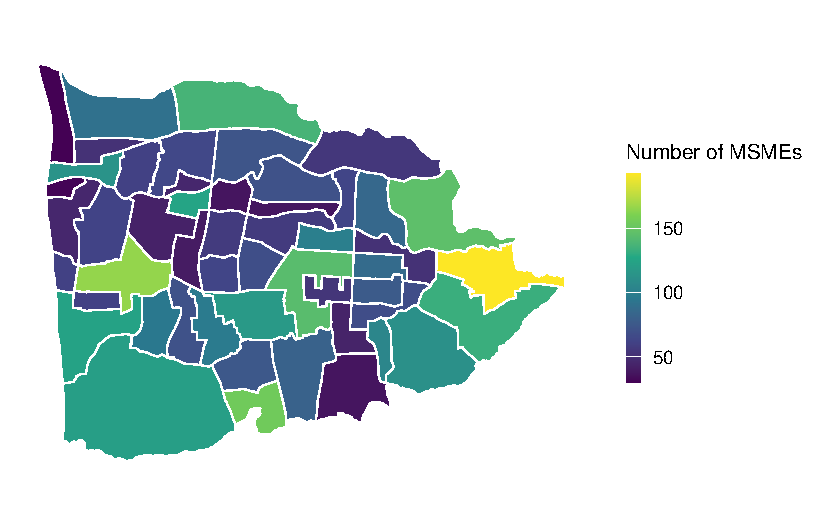
\includegraphics[width=0.75\linewidth,height=\textheight,keepaspectratio]{manuscript_files/figure-pdf/fig-mtrmap-1.pdf}

}

\caption{\label{fig-mtrmap}Map of the 50 urban villages (kelurahan) in
Mataram City, with colour gradients indicating the number of MSMEs in
each village.}

\end{figure}%

Two complementary data sources were used. The first consisted of
administrative or business records containing information on 4,185
MSMEs. These data were used to describe the composition and spatial
distribution of MSMEs in Mataram. The second consisted of survey
responses from 388 MSMEs. The survey data were used to measure digital
readiness and halal-related characteristics.

The combination of these datasets enabled the study to distinguish
between the population-level spatial distribution of businesses and the
more detailed behavioural and perception-based indicators obtained from
the survey.

\subsection{Descriptive analysis of
MSMEs}\label{descriptive-analysis-of-msmes}

Business characteristics were summarised according to business scale,
legal form, location, and economic activity. The dominant economic
activities were identified using the Indonesian Standard Industrial
Classification (KBLI).

Among the 4,185 MSMEs, individually owned businesses constituted the
largest legal category, with 3,560 enterprises or approximately 85.1\%.
Other legal forms included CV, PT, cooperatives, and several less
frequent categories.

\begin{table}[h]

\caption{\label{tbl-summaryumkm}Characteristics of MSMEs by District}

\centering{

\centering\begingroup\fontsize{8}{10}\selectfont

\begin{tabular}[t]{>{\raggedright\arraybackslash}p{2.2cm}>{\centering\arraybackslash}p{1.5cm}>{\centering\arraybackslash}p{2.5cm}>{\centering\arraybackslash}p{2.0cm}>{\centering\arraybackslash}p{1.5cm}>{\centering\arraybackslash}p{1.5cm}>{\centering\arraybackslash}p{1.5cm}>{\centering\arraybackslash}p{1.5cm}}
\toprule
District & Number of MSMEs & Investment (IDR million) & Employment & Micro & Small & Medium & Large\\
\midrule
\cellcolor{gray!10}{Ampenan} & \cellcolor{gray!10}{601} & \cellcolor{gray!10}{10.0 (5.0–50.0)} & \cellcolor{gray!10}{2 (1–2)} & \cellcolor{gray!10}{3 (0.5\%)} & \cellcolor{gray!10}{35 (5.8\%)} & \cellcolor{gray!10}{563 (93.7\%)} & \cellcolor{gray!10}{0 (0.0\%)}\\
Cakranegara & 799 & 15.0 (5.0–50.0) & 2 (1–2) & 12 (1.5\%) & 31 (3.9\%) & 754 (94.4\%) & 2 (0.3\%)\\
\cellcolor{gray!10}{Mataram} & \cellcolor{gray!10}{802} & \cellcolor{gray!10}{20.0 (5.0–50.0)} & \cellcolor{gray!10}{2 (1–2)} & \cellcolor{gray!10}{14 (1.7\%)} & \cellcolor{gray!10}{55 (6.9\%)} & \cellcolor{gray!10}{731 (91.1\%)} & \cellcolor{gray!10}{2 (0.2\%)}\\
Sandubaya & 785 & 20.0 (6.0–50.0) & 2 (1–2) & 11 (1.4\%) & 28 (3.6\%) & 742 (94.5\%) & 4 (0.5\%)\\
\cellcolor{gray!10}{Sekarbela} & \cellcolor{gray!10}{571} & \cellcolor{gray!10}{15.0 (5.0–50.0)} & \cellcolor{gray!10}{2 (1–2)} & \cellcolor{gray!10}{3 (0.5\%)} & \cellcolor{gray!10}{40 (7\%)} & \cellcolor{gray!10}{527 (92.3\%)} & \cellcolor{gray!10}{1 (0.2\%)}\\
\addlinespace
Selaparang & 627 & 15.0 (4.0–50.0) & 2 (1–2) & 3 (0.5\%) & 42 (6.7\%) & 579 (92.3\%) & 3 (0.5\%)\\
\bottomrule
\multicolumn{8}{l}{\rule{0pt}{1em}\textit{Note:}}\\
\multicolumn{8}{l}{\rule{0pt}{1em}Number of MSMEs and business-scale composition are reported as counts (percentages). Investment is reported as median (Q1–Q3), while employment is reported as mean (Q1–Q3).}\\
\end{tabular}
\endgroup{}

}

\end{table}%

The largest groups of business activities included food provision,
specialised retail trade, general retail trade, retail trade in food and
agricultural products, and wholesale trade in food and beverages. These
categories indicate a strong concentration of MSMEs in food-related and
retail activities.

\begin{table}[h]

\caption{\label{tbl-kbli}Distribution of 4,185 MSMEs by three-digit KBLI
business activity group}

\centering{

\centering\begingroup\fontsize{8}{10}\selectfont

\begin{tabular}[t]{>{\raggedright\arraybackslash}p{8.5cm}>{\centering\arraybackslash}p{2.0cm}>{\centering\arraybackslash}p{2.0cm}}
\toprule
Business Activity Group & Number (n) & Percentage (\%)\\
\midrule
\cellcolor{gray!10}{Penyediaan makanan} & \cellcolor{gray!10}{935} & \cellcolor{gray!10}{22.3}\\
Perdagangan eceran khusus & 684 & 16.3\\
\cellcolor{gray!10}{Perdagangan eceran berbagai macam barang} & \cellcolor{gray!10}{674} & \cellcolor{gray!10}{16.1}\\
Perdagangan eceran makanan dan hasil pertanian & 381 & 9.1\\
\cellcolor{gray!10}{Perdagangan besar makanan dan minuman} & \cellcolor{gray!10}{243} & \cellcolor{gray!10}{5.8}\\
\addlinespace
Perdagangan eceran peralatan rumah tangga & 166 & 4.0\\
\cellcolor{gray!10}{Perdagangan eceran kaki lima dan los pasar} & \cellcolor{gray!10}{165} & \cellcolor{gray!10}{3.9}\\
Perdagangan besar barang keperluan rumah tangga & 133 & 3.2\\
\cellcolor{gray!10}{Perdagangan besar berbagai macam barang} & \cellcolor{gray!10}{121} & \cellcolor{gray!10}{2.9}\\
Penyediaan minuman & 117 & 2.8\\
\addlinespace
\cellcolor{gray!10}{Perdagangan besar peralatan khusus} & \cellcolor{gray!10}{79} & \cellcolor{gray!10}{1.9}\\
Aktivitas penatu & 72 & 1.7\\
\cellcolor{gray!10}{Perdagangan eceran hasil pencetakan dan penerbitan} & \cellcolor{gray!10}{62} & \cellcolor{gray!10}{1.5}\\
Perdagangan eceran komputer dan perlengkapannya & 60 & 1.4\\
\cellcolor{gray!10}{Perdagangan suku cadang dan aksesori sepeda motor} & \cellcolor{gray!10}{52} & \cellcolor{gray!10}{1.2}\\
\addlinespace
Perdagangan besar mesin dan peralatan & 44 & 1.1\\
\cellcolor{gray!10}{Perdagangan mobil} & \cellcolor{gray!10}{36} & \cellcolor{gray!10}{0.9}\\
Perdagangan eceran bukan di toko & 33 & 0.8\\
\cellcolor{gray!10}{Perdagangan besar hasil pertanian} & \cellcolor{gray!10}{32} & \cellcolor{gray!10}{0.8}\\
Pembuatan pakaian & 26 & 0.6\\
\addlinespace
\cellcolor{gray!10}{Perdagangan besar atas dasar balas jasa/kontrak} & \cellcolor{gray!10}{26} & \cellcolor{gray!10}{0.6}\\
Perdagangan suku cadang dan aksesori mobil & 20 & 0.5\\
\cellcolor{gray!10}{Jasa boga/katering} & \cellcolor{gray!10}{15} & \cellcolor{gray!10}{0.4}\\
Perdagangan eceran BBM dan LPG & 9 & 0.2\\
\bottomrule
\end{tabular}
\endgroup{}

}

\end{table}%

Spatial visualisation was used to identify the geographical distribution
of businesses and their characteristics across kelurahan

\subsection{Construction of the Digital Readiness
Index}\label{construction-of-the-digital-readiness-index}

The Digital Readiness Index (DRI) was constructed as a composite measure
of the digital readiness of individual MSMEs. The index comprises five
dimensions: \textbf{digital skills, digital business processes, digital
strategy, digital security, and data use}. Each dimension was measured
using multiple Likert-scale questionnaire items. Specifically, digital
skills was measured by three items (SKL1--SKL3), business processes by
three items (BUS1--BUS3), strategy by two items (STR1--STR2), security
by two items (SEC1--SEC2), and data use by two items (DAT1--DAT2).

For MSME \(i\), the score for dimension \(k\) was calculated as the
arithmetic mean of its corresponding questionnaire items:

\[
D_{ik}=\frac{1}{J_k}\sum_{j=1}^{J_k}X_{ijk},
\]

where \(J_k\) denotes the number of items in dimension \(k\). The
overall DRI was then calculated as the arithmetic mean of the five
dimension scores:

\[
DRI_i=\frac{1}{5}\sum_{k=1}^{5}D_{ik}.
\]

Thus, each dimension contributes equally to the overall index,
regardless of the number of items used to measure it. All indicators
were measured on the same Likert scale, so no additional standardisation
was applied. Higher DRI values indicate greater digital readiness.

Two additional composite measures, \textbf{digital infrastructure}
(INF1--INF3) and \textbf{digital commerce activity} (ECO1--ECO3), were
calculated separately but were not incorporated into the DRI. These
measures were subsequently used as explanatory variables in the spatial
regression analysis. At the spatial level, individual DRI scores were
aggregated for each kelurahan using the median, while the number of
surveyed MSMEs was retained as a measure of sample size for each spatial
unit.

\subsection{Explanatory Variables}\label{explanatory-variables}

Four explanatory variables were included in the spatial regression
model: digital commerce activity, digital infrastructure, halal-related
barriers, and halal readiness. These variables were selected to examine
the associations between MSMEs' digital engagement, access to digital
resources, and halal certification-related conditions and the Digital
Readiness Index (DRI) across urban villages (\emph{kelurahan}) in
Mataram City.

Digital commerce activity was measured using three questionnaire items
(ECO1--ECO3), while digital infrastructure was measured using three
items (INF1--INF3). For each respondent, the corresponding score was
calculated as the arithmetic mean of the items within each measure. Both
measures were constructed separately from the DRI, which comprises
digital skills, business processes, digital strategy, digital security,
and data use. This distinction enabled digital commerce activity and
infrastructure to be examined as explanatory factors rather than as
components of the outcome index.

Halal readiness was measured using two questionnaire items (HAL3 and
HAL7), while halal-related barriers were measured using two items (HAL4
and HAL8). The arithmetic mean of the corresponding items was calculated
for each measure. These variables were included to examine whether
perceived readiness for halal certification and reported barriers were
associated with variation in digital readiness.

The four explanatory variables were aggregated to the \emph{kelurahan}
level by calculating their respective means across surveyed MSMEs within
each area. The resulting area-level measures were included as covariates
in the Leroux conditional autoregressive (CAR) model, with the
area-level DRI as the response variable. This specification allowed
associations between the four covariates and digital readiness to be
estimated while accounting for spatial dependence between neighbouring
urban villages.

Let \(Y_{ij}\) denote the Digital Readiness Index (DRI) of respondent
\(j\) in kelurahan \(i\), where \(i=1,\ldots,I\) and \(j=1,\ldots,n_i\).
Let \(\mathbf{x}_{ij}\) denote the vector of individual-level
explanatory variables and \(\mathbf{z}_i\) the vector of kelurahan-level
contextual variables. The multilevel spatial regression model is
specified as

\[
Y_{ij}\mid b_i \sim N(\mu_{ij},\sigma^2),
\]

with

\[
\beta_0
+
\mathbf{x}_{ij}^{\mathsf T}\boldsymbol{\beta}
+
\mathbf{z}_i^{\mathsf T}\boldsymbol{\gamma}
+
b_i.
\]

Here, \(\beta_0\) is the overall intercept, \(\boldsymbol{\beta}\) and
\(\boldsymbol{\gamma}\) are the regression coefficient vectors
associated with individual-level and kelurahan-level covariates,
respectively, and \(\sigma^2\) denotes the individual-level residual
variance. The term \(b_i\) represents the kelurahan-specific random
effect, which accounts for residual heterogeneity between areas and
spatial dependence not explained by the observed covariates.

Spatial dependence in the area-specific effects is modelled using the
Leroux conditional autoregressive (CAR) specification. This formulation
incorporates spatial dependence through the neighbourhood structure of
the kelurahan, with a spatial dependence parameter governing the
relative contribution of neighbouring area effects. It allows the model
to accommodate varying degrees of spatial dependence, from independent
area effects to spatially structured effects, while accounting for
residual heterogeneity across kelurahan.

The Gaussian likelihood is adopted as the primary specification because
the DRI is constructed as a continuous composite index. Its suitability
will be assessed by examining the empirical distribution of the index
and evaluating model adequacy through appropriate residual and posterior
predictive diagnostics. If substantial skewness or boundary
concentration indicates that the Gaussian specification is inadequate,
an alternative likelihood or an appropriate transformation will be
considered.

\subsubsection{Spatial random effects}\label{spatial-random-effects}

The spatially structured variation was modelled using a Leroux
conditional autoregressive (CAR) specification. Let \(u_i\) denote the
spatial random effect associated with area \(i\). Conditional on the
random effects of the remaining areas, the Leroux CAR model can be
expressed as

\[
u_i \mid \mathbf{u}_{-i}
\sim
N\left(
\frac{\rho \sum_j w_{ij}u_j}
{\rho \sum_j w_{ij} + 1-\rho},
\frac{1}
{\tau\left(\rho \sum_j w_{ij}+1-\rho\right)}
\right),
\]

where \(w_{ij}\) denotes the spatial neighbourhood matrix, \(\tau\) is a
precision parameter, and \(\rho\) is the spatial dependence parameter.
The parameter \(\rho\) controls the degree of spatial dependence among
neighbouring areas, with values closer to zero corresponding to weaker
spatial dependence and larger values indicating stronger spatial
structuring.

The spatial neighbourhood structure was defined using queen contiguity
between the 50 kelurahan in Mataram City. Two areas were considered
neighbours when their boundaries or vertices were contiguous. The
resulting neighbourhood structure was incorporated into the Leroux CAR
model to account for spatially structured variation in the DRI that was
not explained by the observed covariates.

The resulting spatial model was estimated using a Bayesian framework.
Posterior inference was obtained using Markov chain Monte Carlo (MCMC),
with multiple chains and burn-in and thinning procedures applied to
reduce the influence of initial values and serial correlation.
Convergence was assessed using standard MCMC diagnostic measures,
including the potential scale reduction factor and effective sample
size.

The Leroux CAR specification was fitted alongside a corresponding
non-spatial Gaussian regression model. Both models used the same
response variable and covariates, allowing the spatial specification to
be evaluated while holding the fixed-effects structure constant.

\section{Results}\label{results}

\subsection{Characteristics of the surveyed
MSMEs}\label{characteristics-of-the-surveyed-msmes}

The descriptive analysis shows that the MSME population in Mataram is
strongly dominated by micro-scale and individually owned enterprises.
The 4,185 business records indicate that the MSME population is not
structurally homogeneous, with substantial differences in business
scale, legal form, and economic activity.

The ten largest KBLI groups were dominated by food provision and retail
activities. Food provision accounted for 935 businesses, or
approximately 22.3\% of the dataset. Specialised retail trade accounted
for 684 businesses (16.3\%), while general retail trade accounted for
674 businesses (16.1\%). Retail trade in food and agricultural products
accounted for 381 businesses (9.1\%), and wholesale trade in food and
beverages accounted for 243 businesses (5.8\%).

This concentration suggests that interventions targeting food and retail
businesses may reach a substantial proportion of the MSME population. At
the same time, the spatial distribution of these businesses indicates
that city-wide averages may conceal meaningful local differences.

\subsection{Digital Readiness}\label{digital-readiness}

The DRI demonstrated considerable variation across the surveyed MSMEs.
The standardised index had a minimum of approximately -1.37 and a
maximum of approximately 2.27, with a median of approximately -0.19. The
distribution indicates that a substantial proportion of businesses were
located below the overall mean of the standardised index, while a
smaller group demonstrated relatively high levels of digital readiness.

At the spatial level, the variation in DRI suggests that digital
readiness is not uniformly distributed across Mataram. This spatial
heterogeneity provides a basis for examining whether neighbouring
kelurahan exhibit similar levels of readiness after controlling for
observed business-related predictors.

\subsection{Digital commerce and halal-related
characteristics}\label{digital-commerce-and-halal-related-characteristics}

Digital commerce activity was positively associated with the DRI and was
also related to infrastructure conditions. This indicates that digital
adoption is not simply a matter of individual business willingness but
is connected to the broader conditions under which businesses operate.

The halal-related indicators showed differentiated relationships with
digital readiness. Halal readiness demonstrated a stronger positive
association with DRI than halal awareness, whereas halal-related
barriers showed a weaker and positive bivariate association before
accounting for the other predictors.

The distinction between readiness and barriers is analytically
important. A business may demonstrate awareness of halal requirements
without having the resources or organisational preparedness required to
implement them. Consequently, policy interventions based solely on
awareness may not adequately address practical constraints.

\subsection{Comparison between GLM and CAR
models}\label{comparison-between-glm-and-car-models}

Both the non-spatial GLM and the Leroux CAR model used the same response
and four predictors:

\[
\mathrm{DRI}
\sim
\mathrm{mean\_ecomm}
+\mathrm{mean\_infr}
+\mathrm{mean\_halbarrier}
+\mathrm{mean\_halreadiness}.
\]

The posterior estimates from the two models were highly similar,
indicating that the inclusion of the spatial component did not
substantially alter the estimated associations between the predictors
and DRI.

\begin{table}[!h]
\centering\begingroup\fontsize{9}{11}\selectfont

\begin{tabular}[t]{>{\raggedright\arraybackslash}p{5.0cm}>{\centering\arraybackslash}p{4.0cm}>{\centering\arraybackslash}p{4.0cm}}
\toprule
Predictor & GLM & Leroux CAR\\
\midrule
\cellcolor{gray!10}{Intercept} & \cellcolor{gray!10}{-1.35 (-3.88, 1.19)} & \cellcolor{gray!10}{-1.36 (-3.90, 1.18)}\\
Digital commerce activity & 0.40 (0.04, 0.75) & 0.40 (0.04, 0.75)\\
\cellcolor{gray!10}{Digital infrastructure} & \cellcolor{gray!10}{0.49 (-0.18, 1.16)} & \cellcolor{gray!10}{0.50 (-0.16, 1.17)}\\
Halal-related barriers & -0.42 (-0.97, 0.13) & -0.42 (-0.97, 0.12)\\
\cellcolor{gray!10}{Halal readiness} & \cellcolor{gray!10}{0.74 (0.24, 1.24)} & \cellcolor{gray!10}{0.74 (0.24, 1.24)}\\
\bottomrule
\end{tabular}
\endgroup{}
\end{table}

The direction and magnitude of the four predictor effects were almost
unchanged between the models. Digital commerce activity showed a
positive association with DRI, with a posterior mean of 0.396 in the CAR
model and a 95\% credible interval of 0.040 to 0.754. Halal readiness
showed the largest positive association, with a posterior mean of 0.737
and a 95\% credible interval of 0.241 to 1.239.

Digital infrastructure also had a positive posterior mean of 0.497,
although its 95\% credible interval included zero (-0.164 to 1.166).
Halal-related barriers had a negative posterior mean of -0.420, with a
95\% credible interval of -0.971 to 0.123. Thus, the posterior intervals
provide stronger evidence for the associations with digital commerce
activity and halal readiness than for the associations with
infrastructure and halal-related barriers.

The similarity between the GLM and CAR estimates is itself informative.
It indicates that accounting for spatial dependence did not
substantially change the estimated fixed effects. Instead, the principal
contribution of the CAR model is to account for geographical structure
remaining in the residual variation.

\subsection{Model fit and spatial
dependence}\label{model-fit-and-spatial-dependence}

The CAR model provided a modest improvement in model fit relative to the
GLM.

\begin{table}[h]

\caption{\label{tbl-modelfit}Model fit comparison between GLM and Leroux
CAR}

\centering{

\centering\begingroup\fontsize{9}{11}\selectfont

\begin{tabular}[t]{lccc}
\toprule
Model & DIC & WAIC & LMPL\\
\midrule
\cellcolor{gray!10}{GLM} & \cellcolor{gray!10}{83.237} & \cellcolor{gray!10}{83.871} & \cellcolor{gray!10}{-42.23}\\
\textbf{CAR} & \textbf{80.474} & \textbf{80.981} & \textbf{-42.01}\\
\bottomrule
\end{tabular}
\endgroup{}

}

\end{table}%

The Leroux CAR model showed modest improvements over the non-spatial GLM
across all three model fit criteria. DIC decreased from 83.24 to 80.47,
while WAIC decreased from 83.87 to 80.98. LMPL also increased slightly,
from −42.23 to −42.01, indicating a small improvement in predictive
performance. These results provide some support for incorporating
spatial structure into the model, although the differences are modest
rather than substantial. The findings suggest that accounting for
spatial dependence provides additional information for explaining
variation in the Digital Readiness Index (DRI), without implying that
the non-spatial model is inadequate.

The estimated Leroux spatial dependence parameter was \[
\rho=0.400
\qquad
(95\%\,CI: 0.016,\;0.916).
\] Because the credible interval is almost entirely within the
admissible range and excludes zero, there is evidence of residual
spatial dependence after accounting for digital commerce activity,
infrastructure, halal-related barriers, and halal readiness.

Here, \(\rho\) should be interpreted as a spatial dependence parameter,
not as an explanatory effect analogous to a regression coefficient. A
value of approximately 0.40 indicates a moderate tendency for
neighbouring kelurahan to exhibit similar residual DRI values. The wide
credible interval, however, indicates substantial uncertainty about the
strength of this dependence.

This result provides statistical justification for retaining the spatial
component in the final model. Neighbouring kelurahan appear to share
some unobserved characteristics associated with DRI that are not
completely captured by the four observed predictors.

\subsection{Interpretation of the fixed
effects}\label{interpretation-of-the-fixed-effects}

The CAR model suggests three important patterns.

First, digital commerce activity has a positive association with DRI.
The posterior mean of 0.396 indicates that kelurahan with greater levels
of digital commerce activity tend to have higher DRI, conditional on the
other predictors and spatial structure. The 95\% credible interval does
not include zero, providing posterior evidence for a positive
association.

Second, halal readiness has the strongest estimated positive association
among the four predictors. Its posterior mean is 0.737, with a 95\%
credible interval of 0.241 to 1.239. This suggests that greater
preparedness for halal-related requirements is associated with higher
digital readiness at the kelurahan level. The result should not be
interpreted causally. Rather, the two dimensions appear to coexist
systematically across the observed areas.

Third, digital infrastructure and halal-related barriers show weaker
posterior evidence. Infrastructure has a positive posterior mean of
0.497, whereas halal-related barriers have a negative posterior mean of
-0.420. However, the credible intervals for both parameters include
zero. These variables therefore show suggestive associations in the
expected directions, but the available data do not provide equally
strong evidence for non-zero effects.

\section{Discussion}\label{discussion}

The results demonstrate that MSME development in Mataram is
multidimensional. Digitalisation cannot be adequately represented by a
single measure of technology adoption, while halal development cannot be
reduced to certification status alone.

The strong representation of food and retail businesses is particularly
relevant to policy design. These sectors are likely to interact directly
with consumers and may therefore benefit from interventions involving
digital promotion, marketplace utilisation, product presentation,
payment systems, and halal assurance.

The positive relationship between digital commerce activity and the
response supports the importance of online channels in MSME development.
However, the result should not be interpreted as evidence that simply
encouraging businesses to create social media accounts will generate
economic improvements. Digital commerce requires supporting
infrastructure, skills, appropriate business strategies, and the ability
to translate digital exposure into actual transactions.

The positive association with infrastructure reinforces this
interpretation. Infrastructure provides an enabling environment within
which digital tools can be used effectively. Consequently, interventions
should not focus exclusively on individual training. Local governments
may also need to address differences in connectivity, access to digital
services, and supporting facilities between administrative areas.

The relationship between halal readiness and the response is also
noteworthy. The result suggests that halal preparedness may be
integrated with broader business development rather than treated solely
as a regulatory obligation. Assistance with certification procedures,
documentation, product assurance, and access to relevant services may
therefore provide benefits extending beyond compliance.

The negative association between halal barriers and the response
provides an additional policy signal. Awareness alone may be
insufficient when businesses face procedural, financial, informational,
or service-access constraints. Interventions should therefore
distinguish between an information deficit and an implementation
barrier.

The spatial model provides an additional perspective. The lower DIC and
slightly improved LMPL indicate that spatial dependence contributes to
explaining the observed variation. This suggests that local policy
design should consider the geographical concentration of MSME
characteristics rather than treating each business as an isolated unit.

However, the spatial effect should not be interpreted as proof that
neighbouring businesses directly influence one another. Spatial
dependence may arise from shared infrastructure, similar market
environments, administrative programmes, population characteristics, or
other unobserved contextual factors.

\subsection{Policy Implications}\label{policy-implications}

The results support a differentiated policy strategy rather than a
single intervention applied uniformly across Mataram.

First, areas with relatively low digital readiness and limited digital
commerce activity should be prioritised for foundational digital
interventions. These may include practical training in social media
marketing, marketplace use, digital payment systems, product
photography, and basic digital business management.

Second, areas with relatively low infrastructure indicators require an
enabling-environment approach. Training is unlikely to be sufficient if
businesses continue to face limitations in connectivity or access to
digital facilities.

Third, areas with low halal readiness but relatively high business
activity may benefit from targeted halal facilitation. Rather than
relying only on general awareness campaigns, assistance can focus on
practical preparation, documentation, product assurance, and navigation
of certification procedures.

Fourth, areas characterised by high halal-related barriers should
receive more intensive facilitation. Local support institutions,
including relevant government agencies and business assistance centres,
can provide direct consultation and help businesses identify and resolve
specific barriers.

Fifth, areas exhibiting multiple disadvantages should be treated as
priority intervention zones. For example, a kelurahan with low digital
readiness, weak infrastructure, low halal readiness, and high barriers
would require an integrated intervention rather than separate programmes
delivered independently.

The spatial analysis therefore supports a policy-zoning framework based
on combinations of characteristics rather than a simple ranking of
kelurahan.

\section{Limitations}\label{limitations}

Several limitations should be considered.

First, the survey component was based on a sample of 388 MSMEs, while
the administrative dataset contained 4,185 business records. The two
datasets therefore provide complementary but not identical
representations of the MSME population.

Second, several indicators were based on self-reported responses. Such
measurements may be affected by differences in interpretation and
reporting behaviour.

Third, the spatial analysis was conducted at the kelurahan level.
Aggregation may conceal substantial within-kelurahan variation. The
results should therefore not be interpreted as applying uniformly to
every business located within an area.

Fourth, the analysis is observational and cross-sectional. The
regression coefficients represent conditional associations and should
not be interpreted as causal effects.

Finally, spatial dependence can be modelled in different ways depending
on the definition of neighbourhood. The present analysis uses queen
contiguity, and alternative spatial structures could potentially produce
somewhat different results.

\section{Conclusion}\label{conclusion}

This study demonstrates the value of integrating MSME profiling,
multidimensional digital and halal indicators, and spatial statistical
modelling for local policy analysis.

The MSME population of Mataram is dominated by individually owned
enterprises and is concentrated in food and retail activities. At the
same time, digital readiness and halal-related characteristics vary
across enterprises and administrative areas.

The CAR model provided a better fit than the corresponding non-spatial
GLM, indicating that spatial dependence contributes information beyond
the observed predictors. Digital commerce activity, digital
infrastructure, and halal readiness were positively associated with the
response, whereas halal-related barriers were negatively associated.

The findings suggest that MSME policy should move beyond uniform
city-wide interventions. Spatially differentiated strategies can be used
to identify areas requiring digital capacity building, infrastructure
support, halal facilitation, or combinations of these interventions.

More broadly, the study illustrates how spatial modelling can support
the transition from descriptive MSME mapping to evidence-based policy
zoning. Future research should extend the analysis using longitudinal
data, finer spatial units, and additional indicators of business
performance to evaluate whether geographically targeted interventions
lead to measurable improvements in MSME outcomes.

\section*{References}\label{references}
\addcontentsline{toc}{section}{References}

\protect\phantomsection\label{refs}
\begin{CSLReferences}{1}{1}
\bibitem[\citeproctext]{ref-anggraini2022assessing}
Anggraini, W., and B. Pranggono. 2022. {``Assessing Digital Readiness of
Small Medium Enterprises: Intelligent Dashboard Decision Support
System.''} \emph{International Journal of Advanced Computer Science and
Applications} 13 (4). \url{https://www.ijacsa.thesai.org/}.

\bibitem[\citeproctext]{ref-adb2021asia}
Asian Development Bank. 2021. \emph{Asia Small and Medium-Sized
Enterprise Monitor 2021}. Asian Development Bank.
\url{https://doi.org/10.22617/SGP210459-2}.

\bibitem[\citeproctext]{ref-bappenas2020rpjmn}
Bappenas. 2020. \emph{Rencana Pembangunan Jangka Menengah Nasional
(RPJMN) 2020--2024}.

\bibitem[\citeproctext]{ref-bappenas2025rpjmn}
Bappenas. 2025. \emph{Ringkasan Rencana Pembangunan Jangka Menengah
Nasional (RPJMN) 2025--2029}.

\bibitem[\citeproctext]{ref-bpsntb2025}
BPS NTB. 2025. \emph{Provinsi Nusa Tenggara Barat Dalam Angka 2025}.
Badan Pusat Statistik Provinsi Nusa Tenggara Barat.

\bibitem[\citeproctext]{ref-chang2021cashless}
Chang, W. L., L. M. Chen, and T. Hashimoto. 2021. {``Cashless Japan:
Unlocking Influential Risk on Mobile Payment Service.''}
\emph{Information Systems Frontiers}, ahead of print.
\url{https://doi.org/10.1007/s10796-021-10160-6}.

\bibitem[\citeproctext]{ref-fajriana2026analisis}
Fajriana, Sappeami, Irwandi, and Masnama. 2026. {``Analisis Kesiapan
UMKM Dalam Implementasi Sertifikasi Halal.''} \emph{Syarikat: Jurnal
Rumpun Ekonomi Syariah} 9 (1): 200--212.
\url{https://doi.org/10.25299/syarikat.2026.vol9(1).27940}.

\bibitem[\citeproctext]{ref-hartini2024implikasi}
Hartini, and Malahayatie. 2024. {``Implikasi Sertifikat Halal Dalam
Manajemen Bisnis Industri Makanan Dan Minuman.''} \emph{--} 1 (2):
116--29.

\bibitem[\citeproctext]{ref-morisson2025digitalisasi}
Morisson, B., and A. A. H. S. Fikri. 2025. {``Digitalisasi UMKM Sebagai
Strategi Meningkatkan Daya Saing Di Era Ekonomi Digital.''}
\emph{E-BISNIS: Jurnal Ilmiah Ekonomi Dan Bisnis} 18 (1): 289--99.
\url{https://doi.org/10.51903/e-bisnis.v18i1.2215}.

\bibitem[\citeproctext]{ref-nabila2023sertifikasi}
Nabila, R., Syukron Jayadi, M. Rusman Hadi, R. Fitrianingsih, and A.
Sukron Haekal Ramdani. 2023. {``Sertifikasi Halal Bagi Produk UMKM Di
Desa Nyurlembang, Kabupaten Lombok Barat.''} \emph{Journal of Applied
Community Engagement} 3 (2): 63--68.
\url{https://doi.org/10.52158/jace.v3i2.639}.

\bibitem[\citeproctext]{ref-oecd2018sme}
OECD. 2018. \emph{SME and Entrepreneurship Policy in Indonesia 2018}.
OECD Studies on SMEs and Entrepreneurship. OECD Publishing.
\url{https://doi.org/10.1787/9789264306264-en}.

\bibitem[\citeproctext]{ref-oecd2021digital}
OECD. 2021. \emph{The Digital Transformation of SMEs}. OECD Studies on
SMEs and Entrepreneurship. OECD Publishing.
\url{https://doi.org/10.1787/bdb9256a-en}.

\bibitem[\citeproctext]{ref-okfalisa2021measuring}
Okfalisa, O., W. Anggraini, G. Nawanir, S. Saktioto, and K. Y. Wong.
2021. {``Measuring the Effects of Different Factors Influencing on the
Readiness of SMEs Towards Digitalization: A Multiple Perspectives Design
of Decision Support System.''} \emph{Decision Science Letters} 10 (3):
425--42. \url{https://doi.org/10.5267/j.dsl.2021.1.002}.

\bibitem[\citeproctext]{ref-pirola2019digital}
Pirola, F., C. Cimini, and R. Pinto. 2019. {``Digital Readiness
Assessment of Italian SMEs: A Case-Study Research.''} \emph{Journal of
Manufacturing Technology Management} 31 (5): 1045--83.
\url{https://doi.org/10.1108/JMTM-09-2018-0305}.

\bibitem[\citeproctext]{ref-purwati2024pendampingan}
Purwati, D., B. Mulianah, E. Agustin, M. Sari, and S. Hidayani. 2024.
{``Pendampingan Pengisian SJPH Melalui Digitalisasi Dan Registrasi
Sihalal Bagi UMKM Desa Wisata Hijau Bilebante Kabupaten Lombok
Tengah.''} \emph{--} 9 (4): 1239--53.

\bibitem[\citeproctext]{ref-rafiah2022digital}
Rafiah, K. K., S. Widianto, I. Kamal, A. Shofiana, A. M. Fajar, and A.
A. Rudini. 2022. {``Digital Readiness of SMEs: An Insight from
Indonesia.''} \emph{AFEBI Management and Business Review} 7 (1): 12.
\url{https://doi.org/10.47312/ambr.v7i01.517}.

\bibitem[\citeproctext]{ref-rahayu2023mapping}
Rahayu, E. S., Sucipto, and S. A. Mardiyani. 2023. {``Mapping the Halal,
Safety, and Quality Food Industry for Micro and Small Enterprises in
Pasuruan Regency.''} \emph{Global Journal Al Thaqafah}, 77--89.
\url{https://doi.org/10.7187/GJATSI072023-7}.

\bibitem[\citeproctext]{ref-uu2014jaminan}
Republik Indonesia. 2014. \emph{Undang-Undang Republik Indonesia Nomor
33 Tahun 2014 Tentang Jaminan Produk Halal}.

\bibitem[\citeproctext]{ref-silva2023clarification}
Silva, R., H. S. Mamede, and V. Santos. 2023. {``Clarification of the
Present Understanding of the Assessment of an Organization's Digital
Readiness in SMEs.''} \emph{Emerging Science Journal} 7 (6): 2279--307.
\url{https://doi.org/10.28991/ESJ-2023-07-06-025}.

\bibitem[\citeproctext]{ref-supriyanto2017klasterisasi}
Supriyanto, A., and J. A. Rozaq. 2017. {``Klasterisasi UMKM Dan Potensi
Wilayah Berbasis Peta Sebagai Strategi Pengembangan Ekonomi Daerah.''}
\emph{Jurnal Pekommas} 2 (2): 143--50.

\bibitem[\citeproctext]{ref-worldbank2021indonesia}
World Bank. 2021. \emph{Indonesia Economic Prospect: Boosting the
Recovery}. World Bank.

\end{CSLReferences}




\end{document}
